\documentclass{beamer}
\usepackage[utf8]{inputenc}
\usepackage{graphicx}
\usepackage{amsmath}
\usepackage{booktabs}
\usepackage{textcomp}
\usepackage{multirow}
\usepackage{color}
\usepackage[ngerman]{babel}
\usetheme{Dresden}
\title{Moose FS}
\author{Ralph Krimmel}

\begin{document}

\section{Einleitung}
\subsection*{}
\begin{frame}
	\maketitle
\end{frame}

\begin{frame}
	\frametitle{Verteilte Dateisysteme}
	\begin{columns}
	\column{.55\textwidth}
	\begin{block}{Viele bekannte Namen}
	\begin{itemize}
		\item Ceph
		\item Lustre
		\item Glusterfs
		\item ...
	\end{itemize}
	\end{block}
	\column{.45\textwidth}
	
\includegraphics[scale=0.22]{ceph.jpg}

	
\includegraphics[scale=0.2]{lustre.png}
	
	
\includegraphics[scale=0.2]{gluster.jpg}
	\end{columns}
\end{frame}

\begin{frame}
	\frametitle{Plattformen}
	\begin{block}{Clients (aka mfsmount): Alle mit funktionierender FUSE Implementierung}
	\begin{itemize}
		\item Linux (ab Version 2.6.14)
		\item FreeBSD
		\item OpenSolaris
		\item MacOS X
	\end{itemize}
	\end{block}
	\begin{block}{Nur Server, Metalogger und Chunkserver}
	\begin{itemize}
		\item Solaris 
		\item Windows mit Cygwin
	\end{itemize}
	\end{block}
\end{frame}

\begin{frame}
	\frametitle{Eher unbekannt: Moosefs}
	\begin{columns}	
	\column{.45\textwidth}
	
\includegraphics[scale=0.5]{moosefs.jpg}
	\column{.55\textwidth}
	\begin{block}{Standard Features}
		\begin{itemize}
			\item Hierarchisch (Baumstruktur)
			\item POSIX Datei Attribute:
			\begin{itemize}
				\item POSIX Rechte
				\item Last Access Time
				\item Modification Time 
			\end{itemize}	
			\item Spezialdateien
			\begin{itemize}
				\item Pipes
				\item Sockets
				\item Blockdevices
			\end{itemize}
			\item Symbolische und Hardlinks
		\end{itemize}
	\end{block}	
	\end{columns}
\end{frame}

\begin{frame}
	\frametitle{Eher unbekannt: Moosefs}
	\begin{columns}	
	\column{.45\textwidth}
	
\includegraphics[scale=0.5]{moosefs.jpg}
	\column{.55\textwidth}
	\begin{block}{Weitere Features}
		\begin{itemize}
			\item 
		\end{itemize}
	\end{block}	
	\end{columns}
\end{frame}


\section{MFS Technik}
\subsection*{}
\begin{frame}
	\frametitle{Lesen}
	\centering
	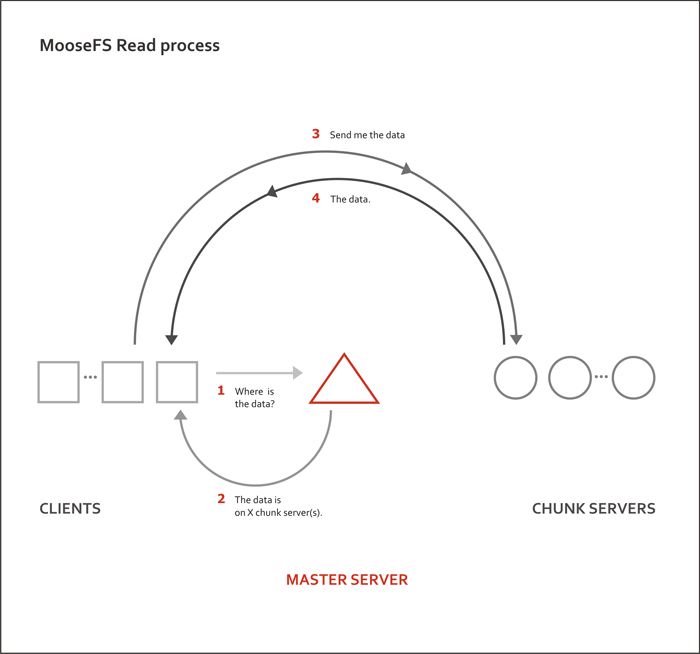
\includegraphics[scale=0.3]{read.png}
\end{frame}

\begin{frame}
	\frametitle{Schreiben}
	\centering
	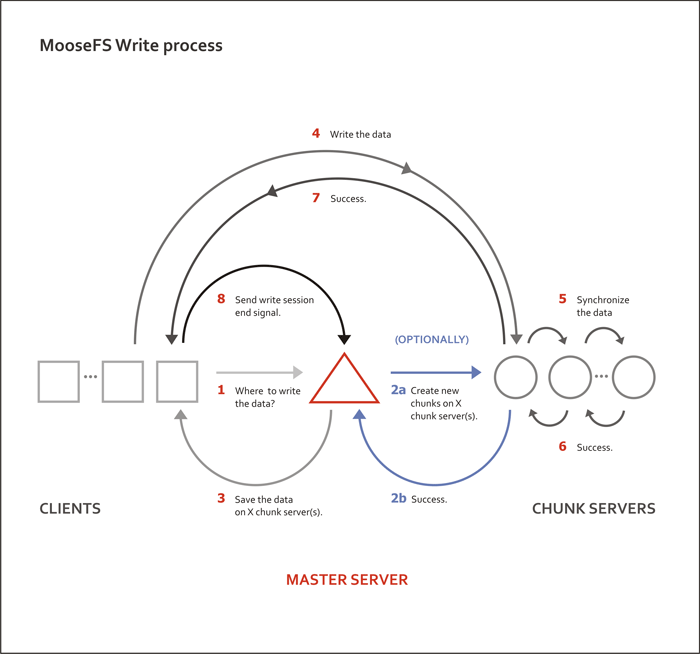
\includegraphics[scale=0.5]{write.png}
\end{frame}




\section{Unstructured data}
\subsection*{}

\begin{frame}
	\frametitle{Definition}
		\begin{itemize}
			\item Unstructured data refers to any data that has no identifiable structure.
		\end{itemize}
\end{frame}


\begin{frame}
	\begin{center}
	\large But there is always a structure!
	\end{center}
\end{frame}

\begin{frame}{Yes, but..}
	\begin{itemize}
		\item Each document itself may have a structure (e.g. HTML)
		\item But: Structure can be not helpful for the processing task
			\begin{description}
				\item In HTML: Tags just for layout, not semantics
			\end{description}
	\end{itemize}

\end{frame}

\begin{frame}
	\frametitle{Examples}
	\begin{description}
		\item Word processing documents
		\item PDF files
		\item E-mail messages 
		\item Blogs and Web pages
		\item Video/Audio
		\item ...
	\end{description}
\end{frame}

\begin{frame}
	\frametitle{Challenges}
	Most of today's data is unstructured (~80\%)
	\begin{block}{Challenges}
	\begin{itemize}
		\item Access to textual data (different file formats)
		\item Language of the data
		\item Volume (See Big Data presentation)
		\item Security of the data
		\item Searchability (the content has to  be understood)
	\end{itemize}
	\end{block}

\end{frame}

\begin{frame}
	\frametitle{Current approaches}
	\begin{itemize}
		\item Manual tagging
		\item Dataminig/Text analytics
		\item Document management systems (e.g. Products from SAS, Provalis Research, Inxight, SPSS)
	\end{itemize}
\end{frame}

\section{Questions?}
\subsection*{}

\begin{frame}
	\frametitle{Questions?}
	\begin{center}
		\large Questions?
	\end{center}
\end{frame}

\end{document}
